%%%%%%%%%%%%%%%%%%%%%%%%%%%%%%%%%%%%%%%%%
% Arsclassica Article
% LaTeX Template
% Version 1.1 (1/8/17)
%
% This template has been downloaded from:
% http://www.LaTeXTemplates.com
%
% Original author:
% Lorenzo Pantieri (http://www.lorenzopantieri.net) with extensive modifications by:
% Vel (vel@latextemplates.com)
%
% License:
% CC BY-NC-SA 3.0 (http://creativecommons.org/licenses/by-nc-sa/3.0/)
%
%%%%%%%%%%%%%%%%%%%%%%%%%%%%%%%%%%%%%%%%%

%----------------------------------------------------------------------------------------
%	PACKAGES AND OTHER DOCUMENT CONFIGURATIONS
%----------------------------------------------------------------------------------------


\documentclass[
11pt, % Main document font size
a4paper, % Paper type, use 'letterpaper' for US Letter paper
oneside, % One page layout (no page indentation)
%twoside, % Two page layout (page indentation for binding and different headers)
headinclude,footinclude, % Extra spacing for the header and footer
BCOR5mm, % Binding correction
]{scrartcl}

%%%%%%%%%%%%%%%%%%%%%%%%%%%%%%%%%%%%%%%%%
% Arsclassica Article
% Structure Specification File
%
% This file has been downloaded from:
% http://www.LaTeXTemplates.com
%
% Original author:
% Lorenzo Pantieri (http://www.lorenzopantieri.net) with extensive modifications by:
% Vel (vel@latextemplates.com)
%
% License:
% CC BY-NC-SA 3.0 (http://creativecommons.org/licenses/by-nc-sa/3.0/)
%
%%%%%%%%%%%%%%%%%%%%%%%%%%%%%%%%%%%%%%%%%

%----------------------------------------------------------------------------------------
%	REQUIRED PACKAGES
%----------------------------------------------------------------------------------------

\usepackage[
nochapters, % Turn off chapters since this is an article        
beramono, % Use the Bera Mono font for monospaced text (\texttt)
eulermath,% Use the Euler font for mathematics
pdfspacing, % Makes use of pdftex’ letter spacing capabilities via the microtype package
dottedtoc % Dotted lines leading to the page numbers in the table of contents
]{classicthesis} % The layout is based on the Classic Thesis style

\usepackage{arsclassica} % Modifies the Classic Thesis package

\usepackage[T1]{fontenc} % Use 8-bit encoding that has 256 glyphs

\usepackage[utf8]{inputenc} % Required for including letters with accents

\usepackage{graphicx} % Required for including images
\graphicspath{{Figures/}} % Set the default folder for images

\usepackage{enumitem} % Required for manipulating the whitespace between and within lists

\usepackage{lipsum} % Used for inserting dummy 'Lorem ipsum' text into the template

\usepackage{subfig} % Required for creating figures with multiple parts (subfigures)

\usepackage{amsmath,amssymb,amsthm} % For including math equations, theorems, symbols, etc

\usepackage{varioref} % More descriptive referencing

\usepackage{listings}



%----------------------------------------------------------------------------------------
%	THEOREM STYLES
%---------------------------------------------------------------------------------------

\theoremstyle{definition} % Define theorem styles here based on the definition style (used for definitions and examples)
\newtheorem{definition}{Definition}

\theoremstyle{plain} % Define theorem styles here based on the plain style (used for theorems, lemmas, propositions)
\newtheorem{theorem}{Theorem}

\theoremstyle{remark} % Define theorem styles here based on the remark style (used for remarks and notes)

%----------------------------------------------------------------------------------------
%	HYPERLINKS
%---------------------------------------------------------------------------------------

\hypersetup{
%draft, % Uncomment to remove all links (useful for printing in black and white)
colorlinks=true, breaklinks=true, bookmarks=true,bookmarksnumbered,
urlcolor=webbrown, linkcolor=RoyalBlue, citecolor=webgreen, % Link colors
pdftitle={}, % PDF title
pdfauthor={\textcopyright}, % PDF Author
pdfsubject={}, % PDF Subject
pdfkeywords={}, % PDF Keywords
pdfcreator={pdfLaTeX}, % PDF Creator
pdfproducer={LaTeX with hyperref and ClassicThesis} % PDF producer
} % Include the structure.tex file which specified the document structure and layout

\hyphenation{Fortran hy-phen-ation} % Specify custom hyphenation points in words with dashes where you would like hyphenation to occur, or alternatively, don't put any dashes in a word to stop hyphenation altogether

%----------------------------------------------------------------------------------------
%	TITLE AND AUTHOR(S)
%----------------------------------------------------------------------------------------

\title{\normalfont\spacedallcaps{Training Project Laboratory Report}} % The article title

%\subtitle{Subtitle} % Uncomment to display a subtitle

\author{\spacedlowsmallcaps{Qianhao Zhang}} % The article author(s) - author affiliations need to be specified in the AUTHOR AFFILIATIONS block

\date{} % An optional date to appear under the author(s)

%----------------------------------------------------------------------------------------

\begin{document}

%----------------------------------------------------------------------------------------
%	HEADERS
%----------------------------------------------------------------------------------------

\renewcommand{\sectionmark}[1]{\markright{\spacedlowsmallcaps{#1}}} % The header for all pages (oneside) or for even pages (twoside)
%\renewcommand{\subsectionmark}[1]{\markright{\thesubsection~#1}} % Uncomment when using the twoside option - this modifies the header on odd pages
\lehead{\mbox{\llap{\small\thepage\kern1em\color{halfgray} \vline}\color{halfgray}\hspace{0.5em}\rightmark\hfil}} % The header style

\pagestyle{scrheadings} % Enable the headers specified in this block

%----------------------------------------------------------------------------------------
%	TABLE OF CONTENTS & LISTS OF FIGURES AND TABLES
%----------------------------------------------------------------------------------------

\maketitle % Print the title/author/date block

\setcounter{tocdepth}{2} % Set the depth of the table of contents to show sections and subsections only

\tableofcontents % Print the table of contents

\listoffigures % Print the list of figures

\listoftables % Print the list of tables

%----------------------------------------------------------------------------------------
%	ABSTRACT
%----------------------------------------------------------------------------------------

\section*{Abstract} % This section will not appear in the table of contents due to the star (\section*)

This is a report for training project laboratory in electrical engineering infocommunication BSc course.
This laboratory consist of two parts, both will be covered by this report.
The first part is circuit realization and measurements around a radio direction 
finder receiver.
The second part is measurements, calculation and software tools realization in Space technology laboratory.

%----------------------------------------------------------------------------------------

\newpage % Start the article content on the second page, remove this if you have a longer abstract that goes onto the second page

\section{Part1 - radio direction finder receiver}

From week 1 to 7 I was working on the radio direction finder receiver. Our task is to realize
the circuit following the schematic. The printed circuit board(PCB) is prepared in advance.

\subsection{Components}
\paragraph{surface mounted components}
All resistors, capacitors, inductors and transistor are packaged using surface mount technology(SMT).
Which makes them tricky to hand solder on the board. When to much soldering is applied
a short circuit could happen between pads underness components. A multimeter is very useful
for troubleshooting.

\paragraph{through hold components}
Audio jack, potentiometer and crystal oscillator are through hold components which provided
a firm connection to the PCB.

\subsection{Circuit design}
The circuit is designed in KiCad

\begin{enumerate}
\item
The radio receiver:\\
	The main blocks:
	\begin{itemize}
	\item 9 turns from 210 cm CuZ copper wire as antenna,
	\item RF (radiofrequency) amplifier,
	\item RF band pass filter,
	\item BJT (bipolar junction transistor) based mixer,
	\item local oscillator,
	\item audio frequency low pass filter,
	\item audio amplifier.
	\end{itemize}
\item
The test transmitter:\\
	Collpitts type oscillator, where the quartz frequency is some 100 Hz different from the receiver local oscillator frequency, in order to make audio signal and it can be heard.
\end{enumerate}

\newpage
\subsubsection{Schematic}

The schematic diagram of the receiver is in Fig. \ref{fig:schematic}.

\begin{figure}[h!]
\centering
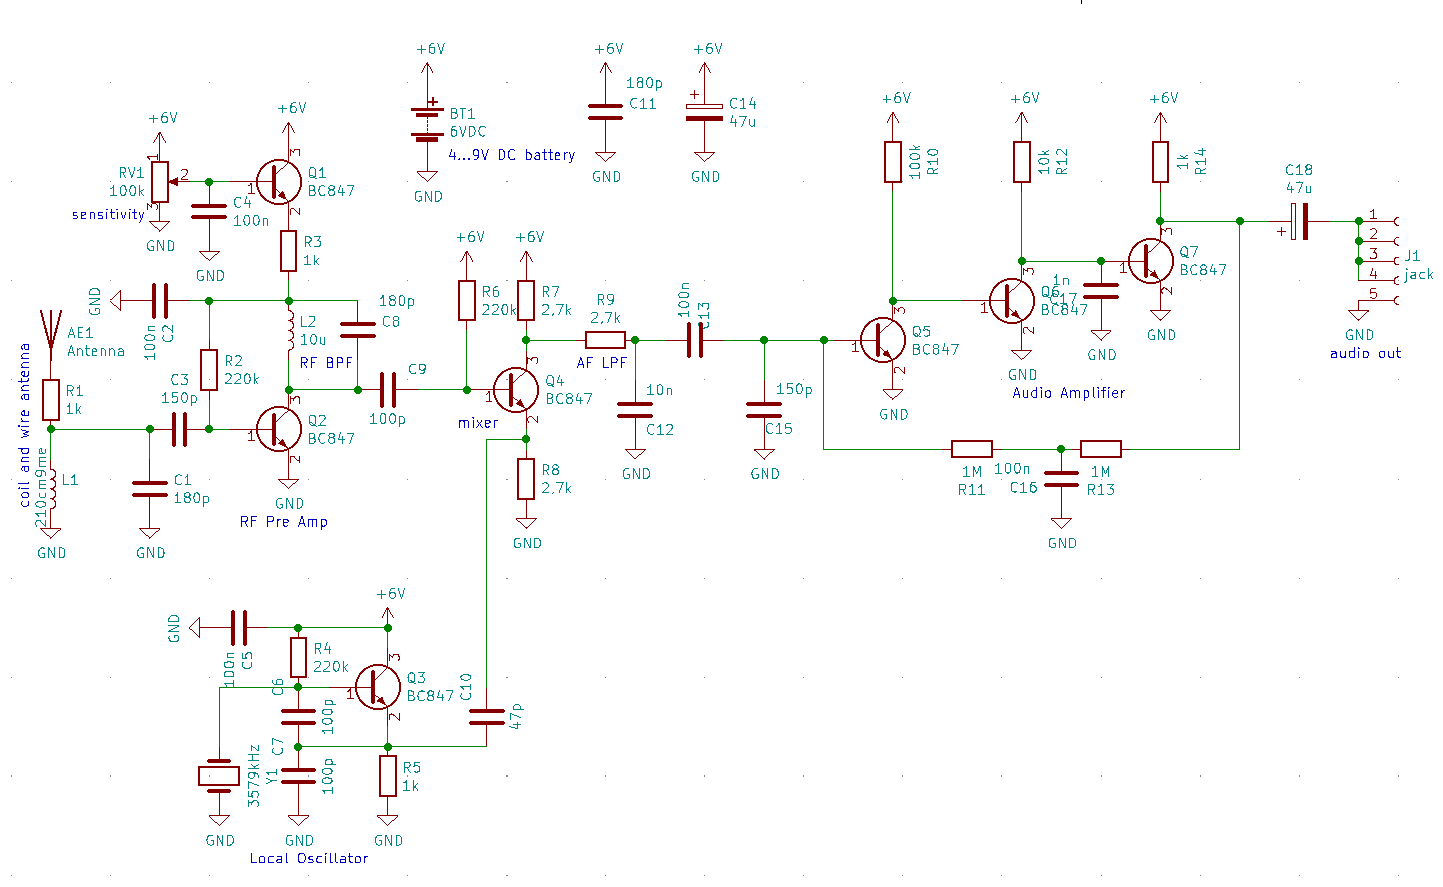
\includegraphics[width=1\textwidth]{sch.png}\\
\caption{Schematic}
\label{fig:schematic}
\end{figure}

\newpage
\subsubsection{Printed Circuit Board}

The designed PCB can be seen in Fig. \ref{fig:pcb}. There are THT and SMD type components.

\begin{figure}[h!]
\centering
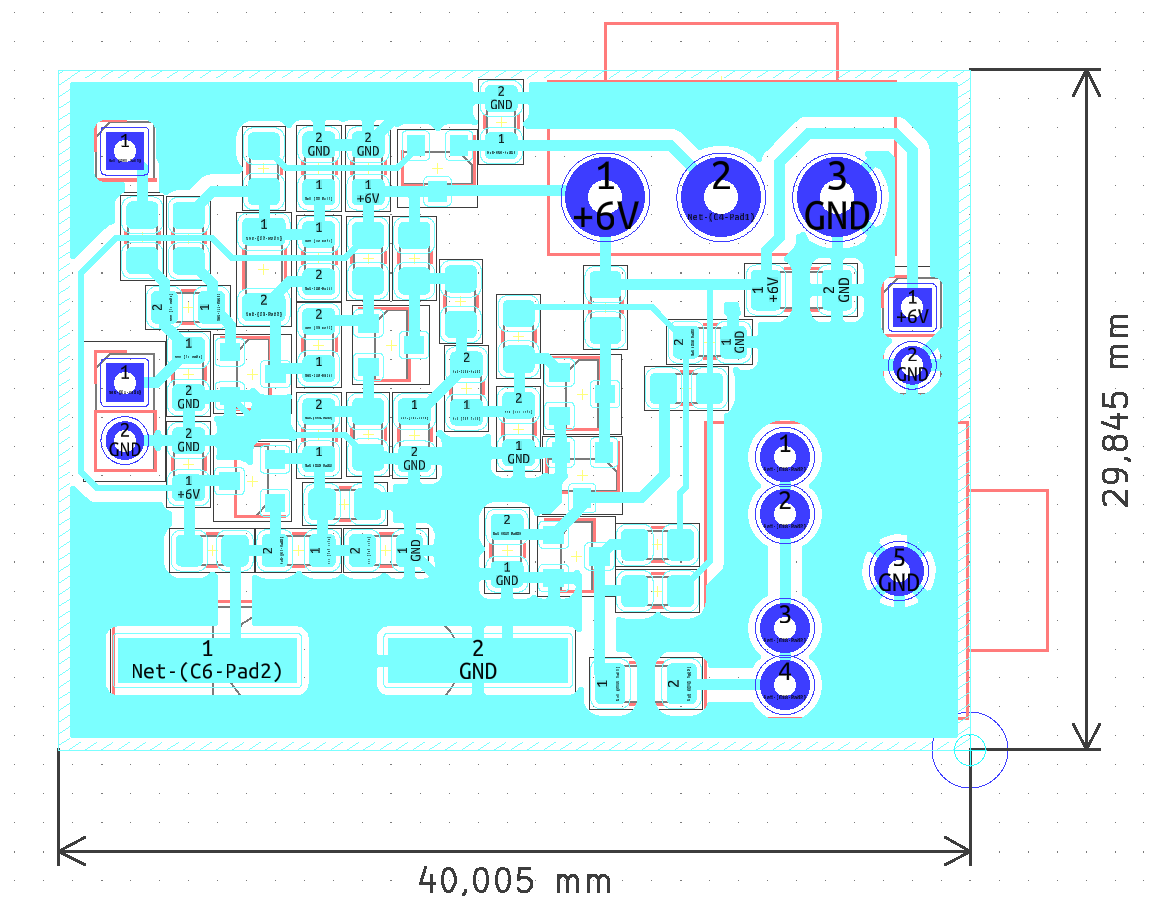
\includegraphics[width=0.7\textwidth]{pcb.png}
\caption{PCB}
\label{fig:pcb}
\end{figure}

\subsubsection{Component placement}

The components with its reference is in Fig. \ref{fig:components}.

\begin{figure}[h!]
\centering
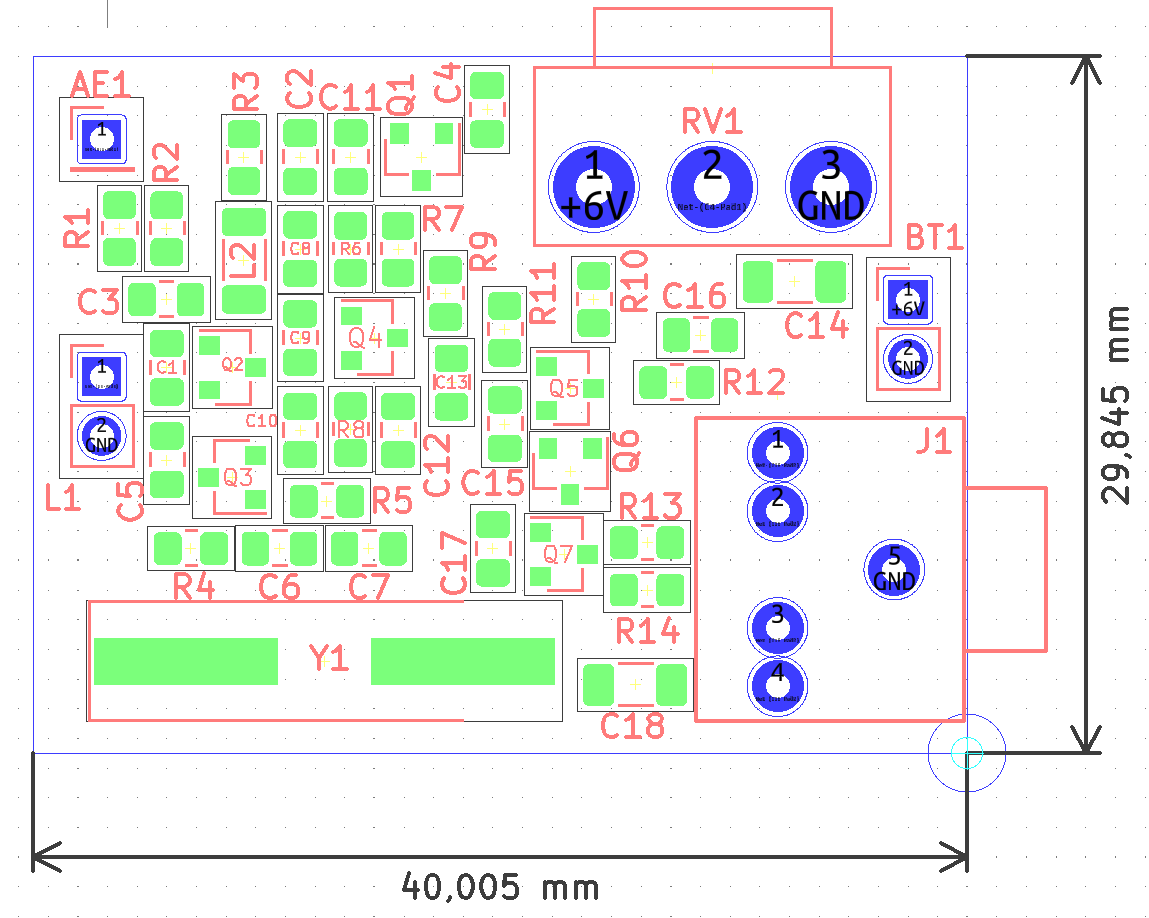
\includegraphics[width=0.7\textwidth]{pos.png}
\caption{Components Placement}
\label{fig:components}
\end{figure}
%------------------------------------------------

\newpage
\subsection{Measurements}
The task is to measure the following parameters of the realized circuit and make test and measurement report based on the measurement results.

\begin{enumerate}
\item Bias DC voltages to the reference GND point on all pins of all semiconductors.
\item Voltage curve in time of the local oscillator output (emitter): peak-to-peak voltage and frequency.
\item Receiver audio (time domain) output signal on the AF output connector: 
variable resistor low, middle, high position: 
peak-to-peak voltage, frequency, curve. During this measurement, 
a single test transmitter will be run near to the receiver.
\end{enumerate}

\subsubsection{Bias DC voltage of transistors}
DC voltage is measured reference to ground. And potentiometer is set to
a low position during measurements.


\begin{table}[h]\centering
    \begin{tabular}{|l|l|}
        \cline{1-2}
        Transistor & Voltage \\
        \cline{1-2}
        Q1 & 807mV \\
        Q2 & 72.4mV \\
        Q3 & 2.79V \\
        Q4 & 1.94V \\
        Q5 & 96.5mV \\
        Q6 & 97.2mV \\
        Q7 & 96.9mV \\
        \cline{1-2}
    \end{tabular}
    \caption{Transistor voltage measurement}
\end{table}

\newpage

\subsubsection{Voltage curve in time domain of the local oscillator output}
In this measurement 10x probe gain is used. I used the quick measure function
on the oscilloscope.

\begin{figure}[h!]
    \centering
    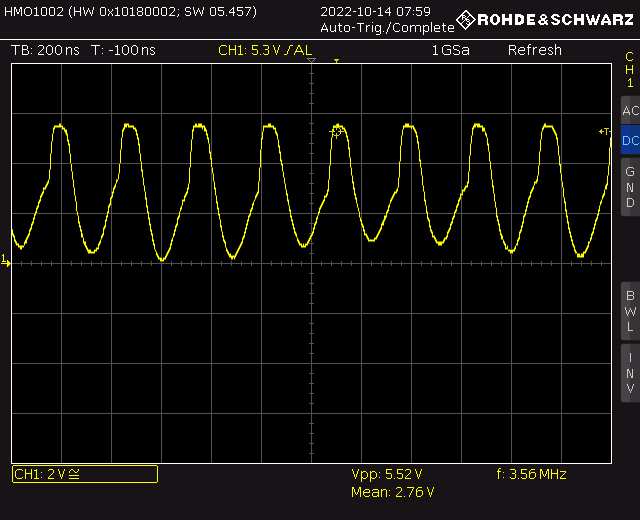
\includegraphics[width=0.9\linewidth]{Figures/BUCK06.PNG}
    \caption{local oscillator output}
    \label{fig:local oscillator output}
\end{figure}

From the schematic \ref{fig:schematic} we can see that a crystal oscillator with 3.579MHz frequency is used.
Our measurement result matches this value within $0.5\%$ of error.


\newpage
\subsubsection{Receiver audio (time domain) output signal}

\begin{figure}[h!]
    \centering
    \subfloat[Low]{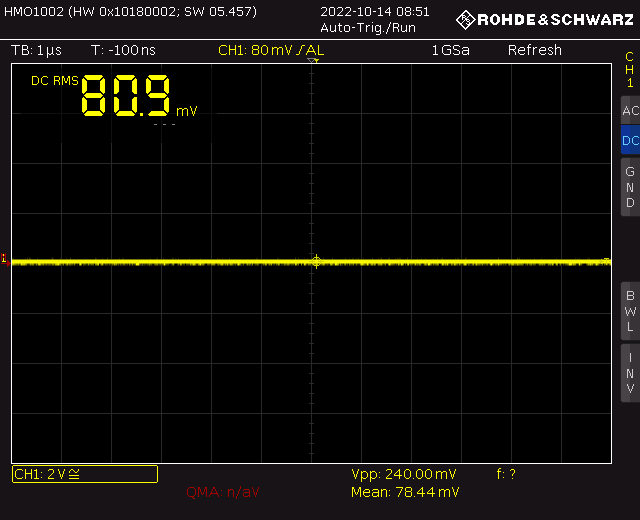
\includegraphics[width=0.4\linewidth]{Figures/BUCK08.PNG}} \quad
    \subfloat[Mid]{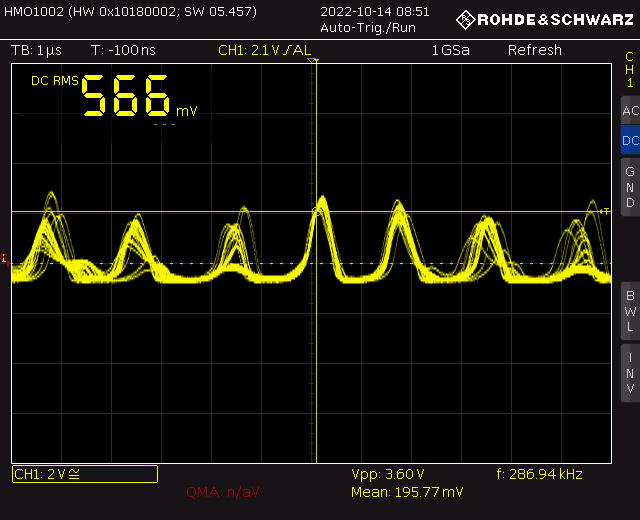
\includegraphics[width=0.4\linewidth]{Figures/BUCK09.PNG}} \\
    \subfloat[High]{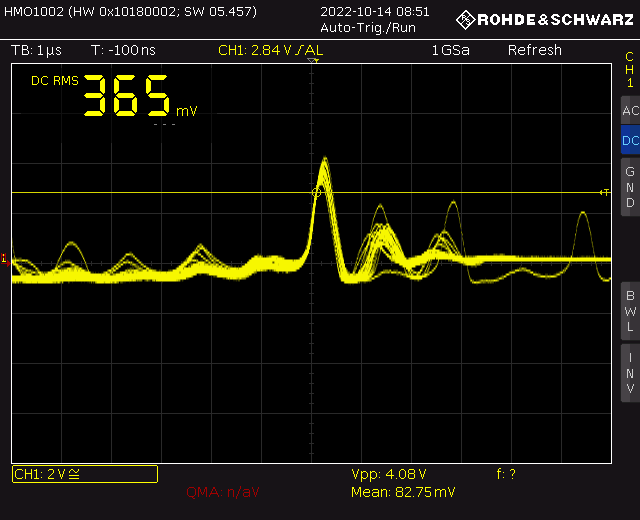
\includegraphics[width=0.4\linewidth]{Figures/BUCK10.PNG}}
 
    \caption{Receiver audio output signal in time domain}
    \label{fig:Receiver audio output}
  \end{figure}

%----------------------------------------------------------------------------------------
%	Part2 - 58Ghz attenuation
%----------------------------------------------------------------------------------------
\newpage

\section{Part2 - 58Ghz attenuation}
From 8 to 14 week I worked for Space technology laboratory supervised by Dr. László Csurgai-Horváth.
Our topic is to research about oxygen and rain attenuation on 58GHz radio signal.

\subsection{Introduction on 58GHz band}
Signal around 60Ghz band has a unique advantage. Around this frequency
signal propagation is effected by oxygen molecule in the air. This phenomenon is 
called oxygen attenuation. Because such phenomenon, signal can not propagate for long distance.
In urban area where high bandwidth communication is required this property can increse
frequency reuse rate which will conserve frequency band resource.

\subsection{Experiment setup}
Two antennas are placed on the roof of building V1 and building E.
An indoor unite was set in the laboratory for data logging.

\paragraph{Geometry}
Geolocation of antennas are measured using GPS coordinate where distance and
elevation angle can be calculated.
GPS coordinates are:
\begin{itemize}
    \item Building V1 antenna: 47.476647, 19.056420, 123.2m
    \item building E antenna: 47.477423, 19.057490, 146.8m
\end{itemize}

From above data we calculated distance $d = 118.0m$ 
and elevation angle $\theta = 11.537^\circ$

\paragraph{Hardware specification}
Testing divices are consist of indoor and outdoor units. Both manufactured by 
Nokia Network. Hardware specification are 
defined in the user manual of these units \cite{metrohopper}
\begin{itemize}
    \item Frequency: 57.725GHz
    \item Polarization: vertical
    \item Antenna gain: 34dB
    \item Transmitter output power: 5dBm
\end{itemize}

\newpage
\subsection{Calculations}
\paragraph{Free space loss}
Free space loss is the loss when signal travels through open space with no
other attenuation. This can be calculated using following equation \cite{openspace}

\begin{equation}
    a_{sz}^{[dB]} = 32.44 + 20log f^{[MHz]}+20log d^{[km]} - G_{TX}^{[dB]} - G_{RX}^{[dB]}
    \label{eq:openspace}
\end{equation}

Where:
\begin{itemize}
    \item $a_{sz}$ is free space loss in dB
    \item $f$ is radio frequency in MHz
    \item $d$ is distance between transmitter and receiver in km 
    \item $G_{TX}$ is transistor antenna gain in dB
    \item $G_{RX}$ is receiver antenna gain in dB
\end{itemize}
\paragraph{Oxygen attenuation}
Oxygen attenuation or Atmospheric attenuation is the effect of signal propagation due to
gas in the atmosphere. The following figure is given in ITU-R P.676 \cite{oxygen} which
demonstrate signal attenuation with different frequency. A peak at around 60GHz is 
clearly visiable which is casued by oxygen molecule in the air.

\begin{figure}[h!]
    \centering
    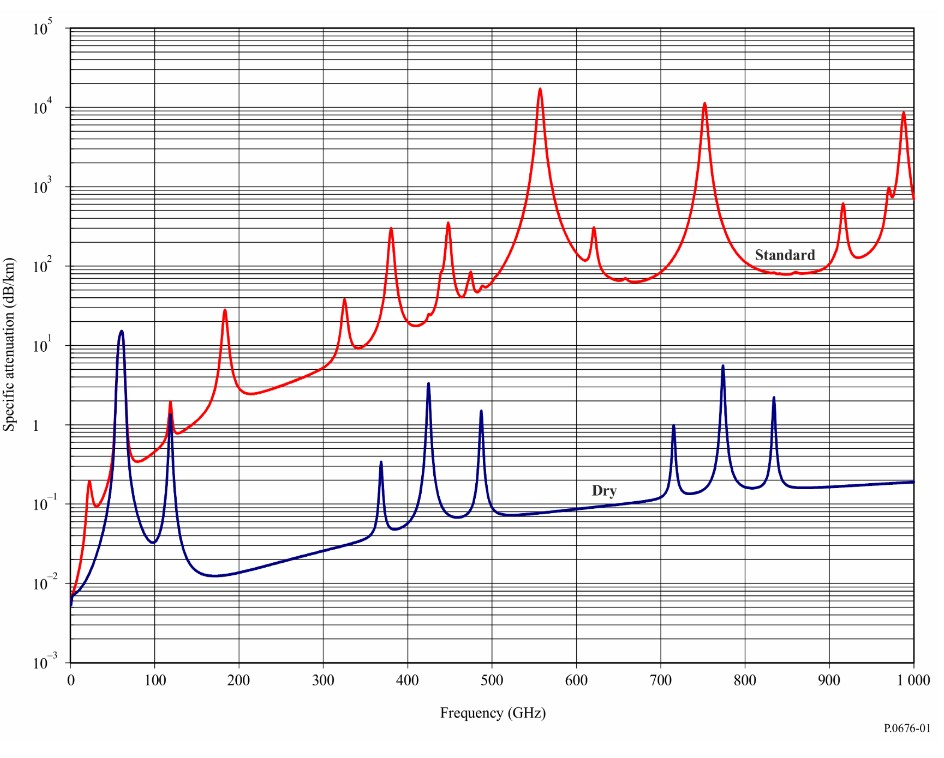
\includegraphics[width=0.9\linewidth]{oxygen.jpg}
    \caption{Atmospheric attenuation}
    \label{fig:Atmospheric attenuation}
\end{figure}

Calculations for oxygen attenuation is quit complicated but for estimation 
purpose Matlab provided a built-in function \verb|gaspl|

\begin{lstlisting}[language=Matlab]
    L = gaspl(range,freq,T,P,den)
\end{lstlisting}
arguments:
\begin{itemize}
    \item range: Signal path length in multimeters
    \item freq: Signal frequency in Hz
    \item T: Ambient temperature in degrees Celsius
    \item P: Dry air pressure in Pa 
    \item den: Water vapor density or absolute humidity in $g/m^3$
\end{itemize}

\paragraph{Rain attenuation}
Rain attenuation is our main research direction. We want to measure how
rain will effect signal propagation on this particular frequency.

%----------------------------------------------------------------------------------------
%	BIBLIOGRAPHY
%----------------------------------------------------------------------------------------
\newpage
\renewcommand{\refname}{\spacedlowsmallcaps{References}} % For modifying the bibliography heading

\bibliographystyle{unsrt}

\bibliography{sample} % The file containing the bibliography

%----------------------------------------------------------------------------------------

\end{document}